\chapter{Modelování vlastností}

Účelem této kapitoly je seznámit čtenáře s problematikou \textit{modelování vlastností} (z angl. \textit{feature modeling}), které je v práci použito jako šablona pro generování zdrojového kódu konfigurátoru.

\section{Motivace}

Motivaci pro modelování vlastností si ukážeme na příkladě. Představme si, že společnost vyvíjí kávovar. Kávovar bude vždy připravovat kávu, avšak jeho vlastnosti se mohou lišit na základě předem určených specifikací. Součástí specifikace může být požadavek, že kávovar bude vyvíjen pro různé trhy, například pro Evropský trh a trh v USA. Dále můze být vyžadováno vytvoření dvou různých edic kávovaru, pro příklad standartní edici a deluxe edici, kde deluxe edice bude oproti standartní edici obsahovat trysku na čistou horkou vodu a displej. Za těchto předpokladů je třeba si uvědomit, že kávovar pro Americký a Evropský trh bude využívat jiný adaptér. Pro Evropský trh je potřeba klasických 220V a pro USA 120V. Zároveň je u kávovaru možno si zvolit, zda bude nebo nebude mít nastavitelné množštví kávových zrn a množství vody, ze které bude káva připravena.

\begin{figure}[H]
	\centering
	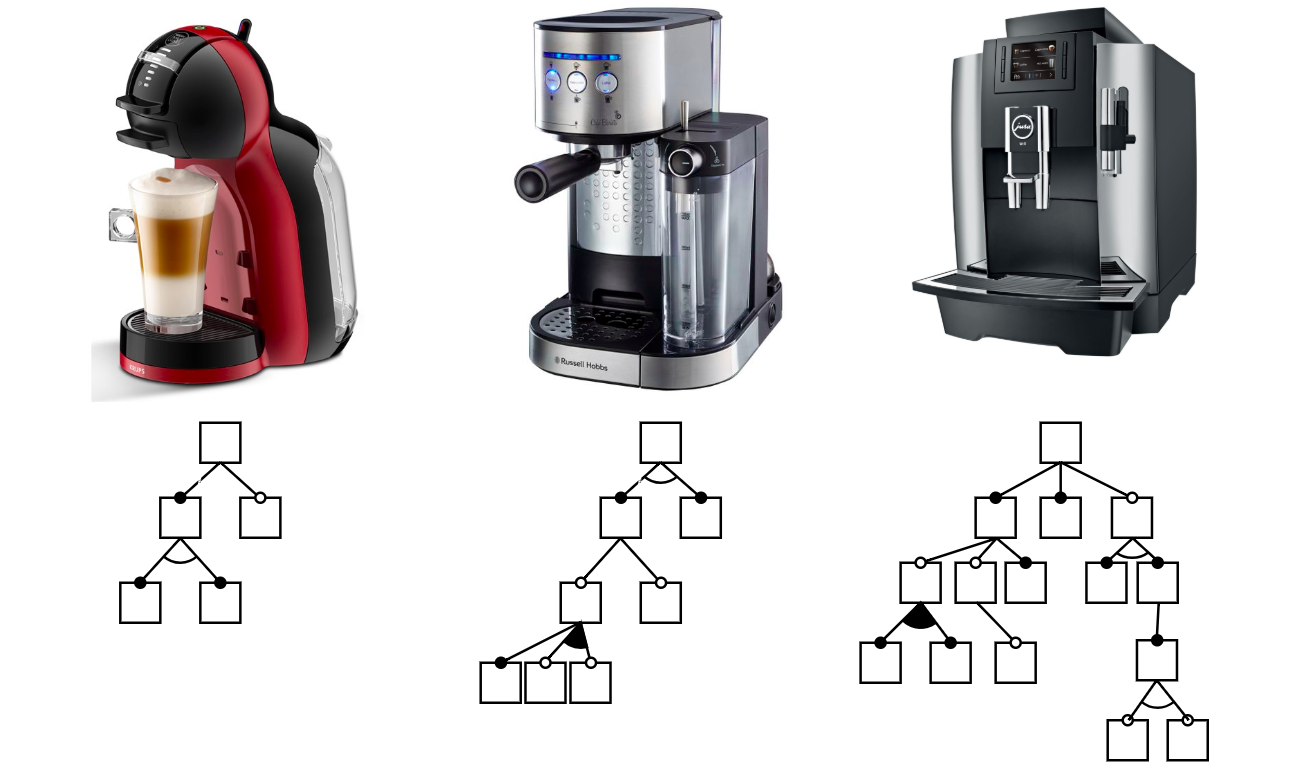
\includegraphics[width=13cm]{images/coffee}
	\caption{příklad různých složitostí diagramů}
\end{figure}


Kávovar se v tomto případě nazývá \textit{produktovou řadou} (z angl. \textit{product line}), \textit{produktovou rodinou} (z angl. \textit{product family}), nebo také \textit{konceptem} (z angl. \textit{concept}). Produktová rodina, či koncept, jsou pojmy, které označují skupinu produktů, které fungují na stejném principu, ale liší se od sebe různými vlastnostmi, tudíž je vytvořeno několik variant. Varianty je třeba spravovat. Je potřeba znázornit, které vlastnosti bude jaká varianta obsahovat, jak na sobě vlastnosti závisí, které a zda jsou potřeba. K tomu nám slouží právě \textit{model vlastností} (z angl. \textit{feature model}).

Model vlastností si také můžeme ukázat na softwarových produktech. Příkladem rodiny produktů může být produkt společnosti Microsoft. Produktovou rodinou je zde například operační systém Windows 10. Windows 10 je vydáván v několika edicích. Těmito edicemi jsou \textit{Home}, \textit{Pro}, a \textit{Enterprise}.
Všechny tyto edice jsou operačním systémem Windows 10, avšak liší se v několika vlastnostech. V tabulce je vidět výčet několika vlastností, ve kterých se operační systémy liší.

\begin{table}[H]
\centering
\begin{tabular}{|c|c|c|c|} 
\hline
\rowcolor[rgb]{0.937,0.937,0.937}  \textbf{Windows}  & \textbf{Home}                                                     & \textbf{Pro}                                                   & \textbf{Enterprise}                                             \\ 
\hline
\textbf{Max. RAM}                                    & \begin{tabular}[c]{@{}c@{}}4GB 32bit\\ 128GB x86-64 \end{tabular} & \begin{tabular}[c]{@{}c@{}}4GB 32bit\\ 2T x86-64 \end{tabular} & \begin{tabular}[c]{@{}c@{}}4GB 32bit\\ 2T x86-64 \end{tabular}  \\ 
\hline
\textbf{Microsoft Edge}                              & Ano                                                               & Ano                                                            & Ano                                                             \\ 
\hline
\textbf{Windows To Go}                               & Ne                                                                & Ano                                                            & Ano                                                             \\ 
\hline
\textbf{DirectAccess}                                & Ne                                                                & Ne                                                             & Ano                                                             \\ 
\hline
\textbf{AppLocker}                                   & Ne                                                                & Ne                                                             & Ano                                                             \\
\hline
\end{tabular}
\caption{Srovnání edicí operačního systému Windows 10}
\end{table}

Tento model je tvořen procesem, který nazýváme modelování vlastností. Vytvořit takovýto model má hned několik výhod. Základní výhodou je přehlednost. Pokud zkonstruujeme správný model vlastností, je v něm na první pohled vidět, jaké produkty můžeme z vlastností sestavit. Model se poté dá použít pro nové verze stejného produktu tím, že se některé vlastnosti změní, nebo také jednoduše přidají.

Hlavní motivací je tedy identifikace a zachycení variability, znovupoužitelnost a rozšířitelnost systému či produktu.

\section{Řada softwarových produktů}

\textit{Řada softwarových produktů} (z angl. \textit{Software product line}) je v softwarovém inženýrství pojem, který označuje kolekci podobných softwarových systémů s podobným zaměřením. Klade důraz na podobnosti mezi softwarovými produkty. Během tohoto procesu je vytvořen koncept, kde lehké odlišnosti vytvoří sadu konkrétních produktů. Nejedná se ale pouze o recyklaci využitelných částí jednoho z hotových produktů, ale o strategické vytvoření základních stavebních kamenů tak, aby byli jednodušše rozšiřitelné a neměnné.

\section{Model rodiny produktů}

\textit{Model rodiny produktů} (z angl. \textit{Family model}) je podle \cite{Pure13} model, který popisuje jak budou výsledné produkty skupiny produktů sestaveny nebo generovány ze specifikovaných částí. Každá komponenta modelu rodiny produktů reprezentuje jeden nebo více funkčních prvků produktu z řady produktů.

\section{Vlastnosti}

Každý koncept má určité \textit{vlastnosti} (z angl. \textit{features}). Pojem vlastnosti můžeme aplikovat jak na vyráběné produkty, tak na různé vlastnosti systému. Příkladem vlastností u vyráběných produktů mohou být vlastnosti znázorněné v příkladu s kávovarem. Vlastnosti jsou také užitečné při vyvíjení softwarových produktů. Požadavkem může být například kompatibilita s různými operačními systémy. Ve výsledném systému bude mít pak každá vlastnost odlišnou implementaci a na základě poskládání těchto vlastností v jeden celek získáme finální systém. Vlastnosti nám tedy zajišťují variabilitu mezi odlišnými produkty se stejným základem.

\subsection{Model vlastností}

Model vlastností znázorňuje závislosti mezi vlastnostmi. Vlastnosti v modelu tvoří strom, kde kořenovou vlastností je koncept. Koncept obsahuje další vlastnosti jako své potomky.

\subsection{Model variant}

\textit{Model variant} (z angl. \textit{Variant model}) je podle \cite{Pure13} model, který z vybraných vlastností modelu vlastností tvoří finální produkt. Jsou v něm zachycené pouze výsledně použité vlastnosti. 

\subsection{Grafické znázornění}
Modely vlastností jsou zobrazovány v \textit{diagramu vlastností} (z angl. \textit{feature diagram}). Diagram vlastností je zakreslován jako stromový graf, kde koncept je kořenovým uzlem a všechny další uzly jsou jeho vlastnostmi. Každý uzel může mít \textit{N} potomků.

\subsection{Typy vlastností}

Jak už bylo řečeno, každý produkt u kterého je požadavek na určitou variabilitu, znovupoužitelnost či rozšiřitelnost obsahuje vlastnosti. Tyto vlastnosti mohou být několika typů. V této části se budeme věnovat základním typům těchto vlastností, tak jak jsou popsány v \cite{Czarnecki98}.

\subsubsection{Povinné vlastnosti}
\textit{Povinné vlastnosti} (z angl. \textit{Mandatory features}) jsou vlastnosti, které výsledný produkt musí obsahovat. Jsou to vlastnosti, na kterých je koncept založen a které jsou zahrnuty v jeho popisu. Povinná vlastnost musí být ve výsledném modelu zahrnuta, pokud je zahrnutý i její rodič. Například náš kávovar bude mít vždy mlýnek na kávu, odkapávač, zásobník zbytků, zásobník vody a další. Bez těchto vlastností se neobejde žádná varianta výsledného produktu. Tyto vlastnosti mají význam hlavně v případě, že jejich rodičovská vlastnost povinná není. Pokud je tedy zahrnut rodič, je nutné zahrnout i tuto vlastnost.

Povinnou vlastnost v diagramu značíme jednoduchou hranou zakončenou vybarveným kruhem.
\begin{figure}[H]
	\centering
	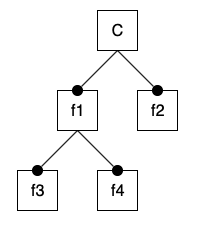
\includegraphics[width=5cm]{images/mandatory}
	\caption{značení povinných vlastností}
\end{figure}

Každá instance konceptu \textit{C} má vlastnost \textit{f1} a \textit{f2} a každá co má \textit{f1} má \textit{f3} a \textit{f4}. Z toho vyplývá, že každá instance konceptu \textit{C} má vlastnosti \textit{f3} a \textit{f4}. Můžeme tedy říct, že koncept \textit{C} je popsán sadou vlastností:

\textit{\{C,f1,f2,f3,f4\}}.


\subsubsection{Volitelné vlastnosti}
\textit{Volitelné vlastnosti} (z angl. \textit{Optional features}) mohou být zahrnuty v popisu konceptu. Jinými slovy, pokud je zahrnut rodič, volitelná vlastnost může a nemusí být zahrnuta. Pokud rodič volitelné vlastnosti zahrnutý není, nemůže být zahrnuta ani volitelná vlastnost na něm závislá. V příkladě s kávovarem může být touto vlastností například zmíněné nastavitelné množství kávových zrn a množství vody. Tuto vlastnost mít kávovar může, ale zároveň nemusí a tvoří tedy další varianty produktu.
Volitelné vlastnosti v diagramu značíme jednoduchou hranou zakončenou prázdným kruhem.
\begin{figure}[H]
	\centering
	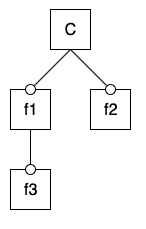
\includegraphics[width=4cm]{images/optional}
	\caption{značení volitelných vlastností}
\end{figure}
Každá instance konceptu může mít vlastnost \textit{f1}, vlastnost \textit{f2}, obě, nebo žádnou. Pokud má vlastnost \textit{f1}, může mít také vlastnosti \textit{f3} a \textit{f4}. Koncept můžeme popsat sadou vlastností: 
\begin{itemize}
	\item \textit{\{C\}}
	\item \textit{\{C,f1\}}
	\item \textit{\{C,f2\}}
	\item \textit{\{C,f1,f2\}}
	\item \textit{\{C,f1,f3\}}
	\item \textit{\{C,f1,f2,f3\}}
\end{itemize}


\subsubsection{Alternativní vlastnosti}
\textit{Alternativní vlastnosti} (z angl. \textit{Optional features}) jsou vlastnosti, kde existuje možnost výběru mezi více vlastnostmi. V kávovaru je takovou vlastností edice, kdy je potřeba si vybrat mezi standart nebo deluxe edicí, ale výsledný produkt nemůže obsahovat obě. Alternativní vlastnosti mohou být volitelné, nebo povinné. Pokud je soubor alternativních vlastností povinný, je třeba vybrat právě jednu z nich. Pokud jsou alternativní vlastnosti volitelné, je třeba vybrat nejvýše jednu z nich.
Alternativní vlastnosti v diagramu značíme prázdným obloukem mezi hranami.
\begin{figure}[H]
	\centering
	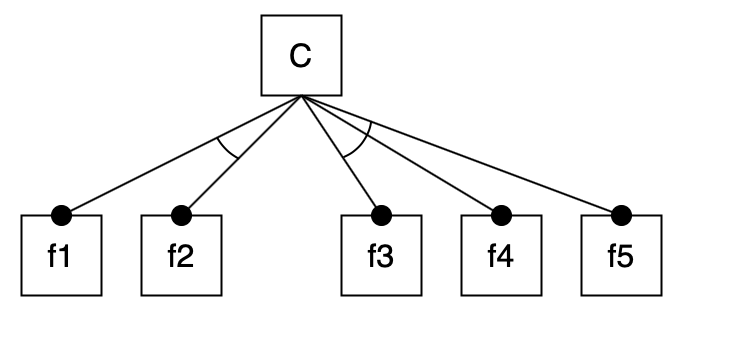
\includegraphics[width=10cm]{images/alternative}
	\caption{značení alternativních vlastností}
\end{figure}
V instanci jsou znázorněný povinné alternativní vlastnosti. Musíme si tedy v levé větvi vybrat mezi vlastnostmi \textit{f1} a \textit{f2} a na pravé větvi mezi vlastnostmi \textit{f3}, \textit{f4} a \textit{f5}. Koncept můžeme popsat sadou vlastností:
\begin{itemize}
	\item \textit{\{C,f1,f3\}}
	\item \textit{\{C,f1,f4\}}
	\item \textit{\{C,f1,f5\}}
	\item \textit{\{C,f2,f3\}}
	\item \textit{\{C,f2,f4\}}
	\item \textit{\{C,f2,f5\}}
\end{itemize}

\subsubsection{Slučitelné vlastnosti}
\textit{Slučitelné vlastnosti} (z angl. \textit{Or-features}) jsou vlastnosti, kde stejně jako u alternativních vlasntostí existuje možnost výběru. Oproti alternativním vlastnostnem ale znázorňují situaci, kdy je možnost výběru více než jedné vlastnosti. Mohou být opět volitené nebo povinné. Pokud je slučitelná možnost volitelná, není třeba vybrat žádnout z nich. Pokud je povinná, je třeba vybrat alespoň jednu z nich. 
Slučitelné vlastnosti v diagramu značíme plným obloukem mezi hranami.
\begin{figure}[H]
	\centering
	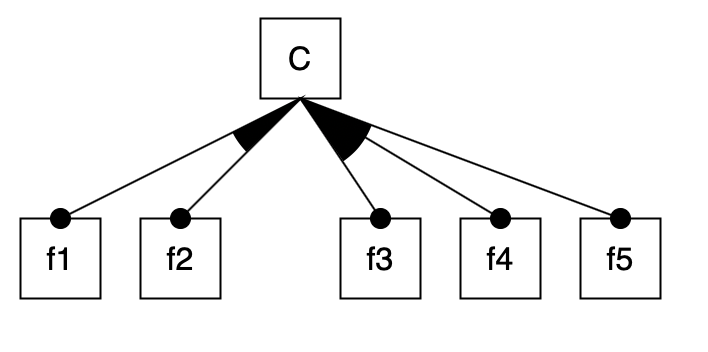
\includegraphics[width=10cm]{images/or}
	\caption{značení slučitelných vlastností}
\end{figure}

\subsubsection{Dalši typy vlastností}
Model vlastností může nabývat velké složitosti. Proto je nutné zavést další typy vlastností a rozšíření původního modelu vlastností. Jedním z těchto rozšíření je zavedení pojmu \textit{kardinalita}. Kardinality označují počet kopíí jednotlivé vlasnosti. Počet těchto vlastností v diagramu označujeme jako interval ve tvaru [\textit{m...n}], kde \textit{m} je dolní a \textit{n} je horní hranice počtu výskytů těchto vlastností. Tato notace se poprvé vyskytla z důvodu inspirace autorů z UML diagramů v publikaci \cite{Rieb02}.

Autoři \cite{Rieb02} také nahrazují alternativní a slučitelné vlastnosti pojmem \textit{skupina vlastností} (z angl. \textit{feature group}). Kardinalita zde označuje kolik vlastností z dané skupiny je možné použít. Alternativní vlastnosti zde nazýváme \textit{XOR skupinou} (z angl. \textit{XOR group}) a slučitelné vlastnosti \textit{OR skupinou} (z angl. \textit{OR group}).

Diagram vlastností dokáže efektivně zachytit veškeré vlastnosti a závislosti mezi nimi. Problém však může nastat v případě, kdy nějaká vlastnost vyžaduje jinou vlastnost, která není jejím přímým rodičem. Pro takové případy je zde zaveden pojem \textit{omezení} (z angl. \textit{constraints}). Tato omezení si můžeme představit u požadavku, že kávovar bude mít displej pouze v případě, že velikost nádrže na vodu bude více než půl litru. Tyto dvě vlastnosti spolu v diagramu nijak nesouvisí a využívají tedy omezení. Omezení mohou být dvojího typu. Podle autorů \cite{Pas05} to jsou \textit{lokální omezení} (z angl. \textit{local constraints}) a \textit{globální omezení} (z angl. \textit{global constraints}). Pojem lokální omezení je používán, pokud se toto omezení vztahuje pouze ke společnému rodiči těchto vlastností. Pojem globální omezení je používán pokud se tato omezení vztahují na vlastnosti napříč diagramem. Tato omezení se budou značit značkou \textit{requires}, pokud vlastnost vyžaduje jinou vlastnost napříč diagramem a značkou \textit{excludes}, pokud tato vlastnost nějakou jinou vlastnost vylučuje.


\subsubsection{Shrnutí}
Na základě těchto typů vlastností dokážeme z libovolného konceptu sestavit hotový model vlastností. Díky němu jsme schopni zachytit veškeré varianty finálního produktu. Jsme schopní zjistit co jaká varianta vyžaduje a co musí obsahovat. 

Diagram by krom názvů vlastností a typu závislostí měl obsahovat i informace o vlastnostech. Tyto informace by měly obsahovat důvod, proč je tato vlastnost vyžadována, jak souvisí se zbytkem modelu a veškeré další informace, které mohou být při vývoji užitečné. 







